\chapter{Experiment}\label{chap:exp}


\section{Set up and instrumentation}

For this measurements, the students will have these materials available at the Laboratory of Nuclear Physics:
	\bi
		\item Scintillators and photomultipliers
		\item Acquisition electronics:
		\bi
			\item Pre-amplifier and amplifier
			\item Scope
			\item Pulse Generator
			\item High voltage power supply
			\item Discriminator
			\item Coincidences module
		\ei
		\item Blocks and layers of absorbent materials
		\item Voltmeters
		\item Wiring
	\ei

	\bfi[H]
		\bc
			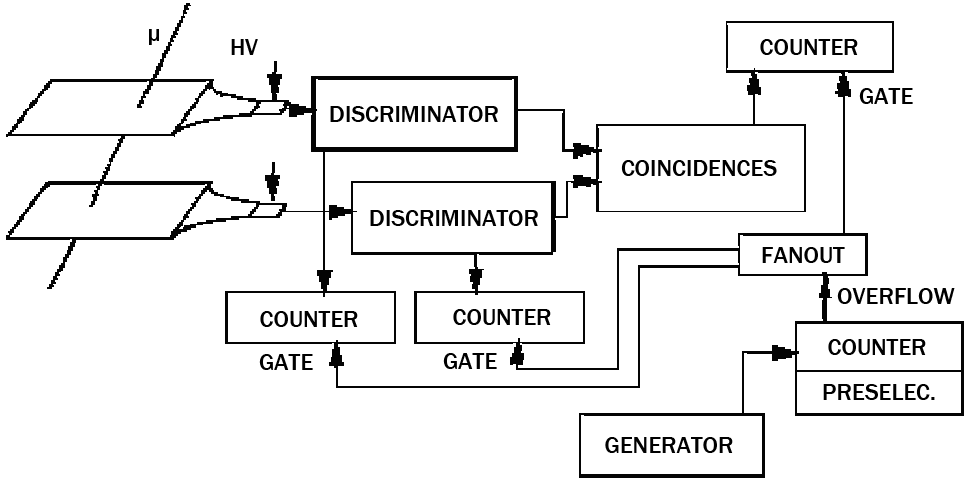
\includegraphics[width=\textwidth]{img/setup.png}\\[12pt]
			\caption[Experimental set up.]{Experimental set up.}\label{fig:setup}
		\ec
	\efi



	\subsection{Scintillators and photomultipliers}

		\subsubsection{Scintillators:} 

			\underline{\textit{Characteristics of the detectors used:}}

			The detectors chosen for this application must be able to withstand a large electric field, and in the absence of radiation, the electric current flow should be minimal or null so that the noise is low. This seems to require an insulating material, but also the e$^-$ should be easily extracted from the atoms, and in great number by the radiation. Also, the  ions must be able to easily travel in the material, which suggests using an electrical \textbf{conductor}. The obvious compromise is what we found in the laboratory: \textbf{a semiconductor}.

There are two basic types of detectors, those composed of \textit{organic} materials (which may be liquid or solid), and those made of \textit{inorganic} materials. The choice of one or the other depends on the type of experiment to be performed. In this case we are looking for a short response time, so the relatively inefficient plastic scintillators are a better choice. In this experiment we have chosen \textbf{organic solid plastic scintillators}.

The properties considered in choosing the material include:

		\bi
			\item \textit{the fraction of incident energy that appears as light}: they can be used in a wide range of energies from 20 keV (e$^-$) to 200 MeV (heavy ions),
			\item \textit{the efficiency} (the probability that the radiation is absorbed) for the active area, the efficiency is 100\%, and its power vs. pulse-height curves are linear over a wide range,
			\item \textit{the response time}: fast pulses emerge and are suitable for short times ($\sim$ 1 ns) with coincidences circuitry,
			\item \textit{the energy resolution}: it is only surpassed by the spectrometers,
			\item \textit{the transparency}: the scintillators are transparent to its own radiation.
		\ei

The dimensions of these scintillators in the laboratory are listed below:

		\bc \textit{\textbf{S}} = (31 cm.) $\times$ (10 cm.) = \textbf{0.031 m$^2$}.\ec

Whenever a reference is made to \textit{\textbf{S}} in this work, this values will be used.

			\noindent\underline{\textit{Operation:}}

In scintillator counters, electrons formed in the ionization process are the same as those of the electronic pulse. The intermediary between the two is the ordinary light.

In organic scintillators, interactions between molecules are weak, and its properties can be understand in terms of discrete excited states of molecules. The electrons can be excited to higher electronic states (jumps between electronic levels) or the atoms of the molecule may start vibrating (jumps between vibrational levels). Typical vibrational energies are of the order of 0.1 eV, whereas the electronic excitation energies are on the order of eV.

		\noindent\begin{minipage}{0.5\textwidth} 
			\hspace*{2ex} The excited electrons are those that are not involved in the binding of the molecule. The incident cosmic radiation interacts with many molecules, losing a few eV (slightly different for hard or soft) in each interaction, exciting them.\\

			\hspace*{2ex} The vibrational states excited with that energy first decay ($\sim$1ps) to the first vibrational ground state of the excited electronic state, which then decays ($\sim$10ns) to one of the vibrational states of the electronic ground state, which in turn decays quickly to its corresponding vibrational ground state.
		\end{minipage}
		\begin{minipage}{0.5\textwidth} 
			\bfi[H]
				\bc
					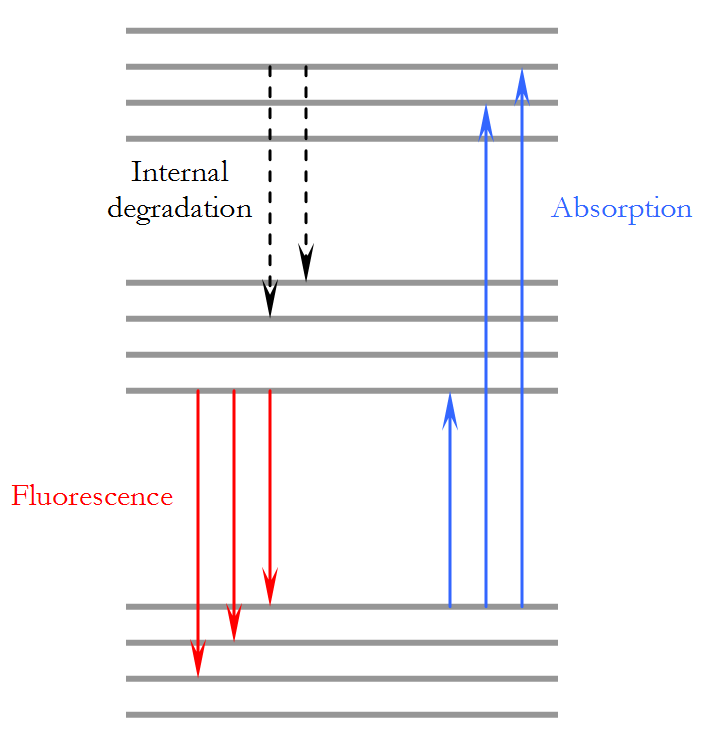
\includegraphics[width=.9\textwidth]{img/scintillator.png}
					\label{fig:molecular}
				\ec
				\caption[Molecular gamma decay.]{Molecular gamma decay.}
			\efi
		\end{minipage}\captionsetup{width=0.8\textwidth}


These transitions can be radiative or non-radiative. In non-radiative, there is light emission (luminescence), which in the case of atoms is around the UV.

Finally, this explains its \textit{transparency}: Under normal circumstances, at room temperature, all of the scintillator molecules are in the lowest vibrational state of the electronic ground state.

At thermal energy (kT = 0.025 eV) the corresponding population follows a \textbf{Boltzmann distribution}: \textit{exp($-$E / kT)}, so it is very unlikely that there are any excited vibrational states at that temperature. This ensures that ONLY ONE of the photons emitted in the many possible transitions has a probability of being absorbed by the scintillator itself.

There are also other processes happening within a scintillator:

	\bi
		\item \textit{Fluorescence Emission} of radiation of a given wavelength by a substance as a result of the absorption of radiation of a shorter wave length. This emission occurs essentially only during irradiation.

		\item \textit{Pair production}: A process for X-radiation and $\gamma$ absorption in which the incident photon is annihilated in the vicinity of the absorbent nucleus of the atom with the subsequent production of a pair e$^-$ / e$^+$. This reaction only occurs for incident photons whose energy exceeds 1.02 MeV.

		\item \textit{Photoelectric Effect}: A process by which a photon removes an e$^-$ of an atom. All the energy of the photon is absorbed in extracting it and giving it kinetic energy.

		\item \textit{Compton effect}: An attenuation process observed for X or $\gamma$ radiation, in which an incident photon interacts with an orbital e$^-$ of an atom to produce a recoil e$^-$ and a scattered photon of lower energy than the incident.
	\ei

		\subsubsection{Photomultipliers (PM):}

		For this experiment, the geometry of the photomultiplier is very different from the geometry of the scintillators. This justifies the use of a light guide between the two.

		The gain of a PM is calculated as:

		\be\frac{number\ of\  e^-\  going\  out}{number\  of\  e^-\  going\ in} \sim 3-4\ee

At the end of \textbf{n} stages, the number of e$^-$ will be N (e$^-$) \textbf{$\sim$ 4$^n$}.

		In the semitransparent photo-cathode, the incident radiation extracts an e$^-$ by photoelectric effect. The photo-cathode is a thin layer of photosensitive material with a work function $\phi$, so that if the frequency of the incident photon is $\nu$, the e$^-$ will exit with an energy of:

	\bc$E = h\nu - \phi$\ec

From this expression it is evident that a minimum $\nu$ is needed for the process to happen. PM quantum efficiency is then defined as:

	\be QE(\lambda) = \frac{photoe^-\ out}{incident\ gammas}\ee

which depends on $\lambda$ and the structure of the material.

		Then they pass through the e$^-$ collector, where there are several focusing electrodes that use an electric field to attract the e$^-$ to the first dynode. This way, the number of e$^-$ reach the dynode from any point of the cathode, and the arrival time is independent of the emission point.

		In the tube of the PM, the e$^-$ are accelerated into a series of secondary electrodes, generating more e$^-$ in each new clash with the dynodes. These are connected to a high voltage source and a series of voltage dividers. Thus, typical potential differences of about 100 V between adjacent dynodes are obtained, and therefore, the electrons impact the dynodes with about 100 eV of energy.

	\bfi[H]
		\bc
			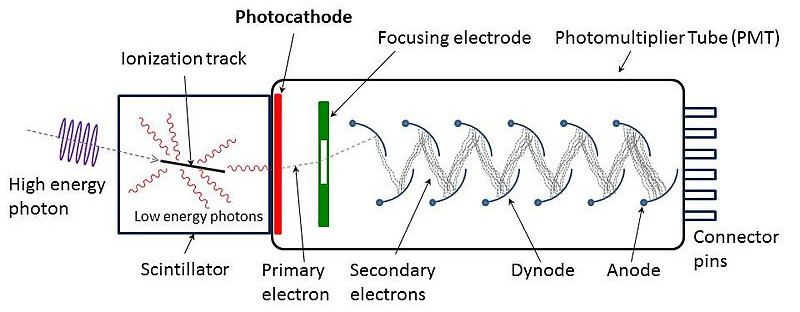
\includegraphics[width=\textwidth]{img/pmtube.jpg}\\[12pt]
			\caption[Schematic view of a photomultiplier.]{Schematic view of a photomultiplier. The electrons released from the cathode are attracted to the first dynode and multiplied. Each successive dynode is at a higher potential than the previous. A typical tube has 10 to 14 dynodes. At each step, the number of electrons is increased by a factor of about 5. \textbf{Image credit:} By Qwerty123uiop (Own work) [CC-BY-SA-3.0 (\scriptsize\href{http://creativecommons.org/licenses/by-sa/3.0}{\textbf{\url{http://creativecommons.org/licenses/by-sa/3.0}}}{\small)], via Wikimedia Commons.}}\label{fig:pmtube}
		\ec
	\efi

The dynodes are made ​​of a material that has a high probability of emitting secondary electrons. Between $10^5$ and $10^7$ e$^-$ are created by each photoe$^-$ emitted by the cathode, and to free an e$^-$ can cost up to 2 or 3 eV. A gain of 30--50 e$^-$ is therefore possible. The amplification depends on the number of dynodes (n) and the voltage between them (V$_{d-d}$).
 
The secondary emission factor is defined as $\delta = k\Delta V_{d-d}$, so the gain will be $G = \delta^n$. Keep in mind that changes of 1\% in $\Delta V_{d-d}$ lead to changes in gain of n\%, which means that HV has to be regulated.

		However, electrons are released in random directions in the material, and relatively few will be actually delivered to the surface, so that a gain of 5 in each dynode is more common. Even so, with a tube 10 dynodes, the total gain will be of 510 ($\sim$107). That is, each time a cosmic ray hits the system, it produces 10,000 \enquote{primary} ionizations in the scintillator, of which about 100 are gammas.

Finally, the cascade of e$^-$ is collected at the anode, and becomes a signal of electric current that can be amplified and analysed.
	   
		When connecting an oscilloscope to a PM in the set up that we have in the laboratory, it will be noted that there is always a \enquote{dark current}, due to the presence of neutrinos, decays at room temperature, etc. Furthermore, with the increase in the threshold voltage of the discriminator, the noise and signal amplitude will increase too.

The joint of the scintillator to the PM is usually done through an optical coupling (silicone oil, light guides, etc.). If we connect a scintillator to a PM, a signal with a pulse of a certain amplitude that appears randomly will be added, this means that a particle has reached the scintillator. In addition, the noise that it had before will be increased by the so-called \enquote{white noise}, which has a flat spectrum and is nothing but the noise of the signal itself. Parasitic currents can appear also. As the voltage (HV) increases, the gain will increase too, and therefore the number of events, but there will come a time when even if the tension rises, no more particles are detected, only noise will be increased.

	\noindent\underline{\textit{Detection process:}}

To summarize, the detection process follows these steps:

	\ben
		\item The incident cosmic radiation interacts with atoms and molecules, exciting the material.
		\item The excited states decay emitting visible (or near visible) light, or fluorescence light.
		\item The light travels through the light guides, and reaches the photosensitive surface of the PM, extracting photoelectrons.
		\item The electrons are accelerated and multiplied, to form an electrical pulse in the photomultiplier tube.
	\een


	\subsection{Acquisition Electronics}

In this measurements, a chassis with rear power supply adapted for NIM (\textit{Nuclear Instrument Module standardized}) modules was used, following the AEC Report TID-20893 standard, which ensures compatibility in size, power and signal level for instruments manufactured by different vendors.

The system for this experiment is already assembled, and includes a set of modules that are used in many experiments: a pre-amplifier, an amplifier, a discriminator, a counter and an oscilloscope. Each module provides a necessary function for the overall system, which according to the diagram in Fig. \ref{fig:setup} is nothing more than a simple \textbf{counting system}. It is important that all the equipment has the same impedance, to avoid signal reflections.

These electronic modules are divided into two general types:

	\bi
		\item \textit{Logic}: Those that generate an output pulse of fixed shape and amplitude if a logical criterion is fulfilled. \textit{Example}: the discriminator, which provides an output pulse (always with the same amplitude) each time it receives an input pulse whose amplitude is greater than the threshold level. The SCA is also logical.

		\item \textit{Linear}: Those in which the linear output signal contains information such as the energy of a detected event (one incident particle that has been absorbed in the detector). The linear signals vary over a range of amplitudes which shows the energy spectrum analysis of the event.
	\ei

It is always important to distinguish between linear and logical connections to mount a NIM equipment. The logic signals are often used to provide timing information and control the function of each instrument in a system.

		\subsubsection{Preamplifier and amplifier:}

Particles produce pulses from the detector whose amplitudes are proportional to the energy of cosmic radiation. The \textbf{preamplifier} and \textbf{amplifier} simply amplify each pulse by a fixed gain factor, and shape the pulse as well.

For example, with a gain factor of 10, if a particle arrives with 5 MeV, a signal of 0.5 V will leave the preamplifier, and a signal of 5 V from the amplifier. So each time a particle of 5 MeV hits the detector, a pulse of 5 V is produced.

The linear signal is the output of the amplifier, and contains information on the energy of the particle that produced the pulse, \textit{i.e.}, the output of the amplifier is proportional to the energy of the absorbed particle. 

		\subsubsection{Discriminator:}


In addition to the information provided by the pulse height, the number of linear signals can also show how many events occurred with a certain pulse amplitude per unit time. If the discriminator is set to 5.1 V for the output of the amplifier, and particles are coming with energies of 5 and 6 MeV, the logical pulse discriminator sends only the particles of 6 MeV. These logic pulses are then sent to the counter and counted.

		\subsubsection{Oscilloscope:}

It is the instrument used to observe the input and output pulses for the modules in the system, and to determine whether the shape of the signals, the amplitudes and timing are correct with respect to the rest of the equipment.

	\bfi[H]
		\noindent\begin{minipage}{0.5\textwidth} 
			\bc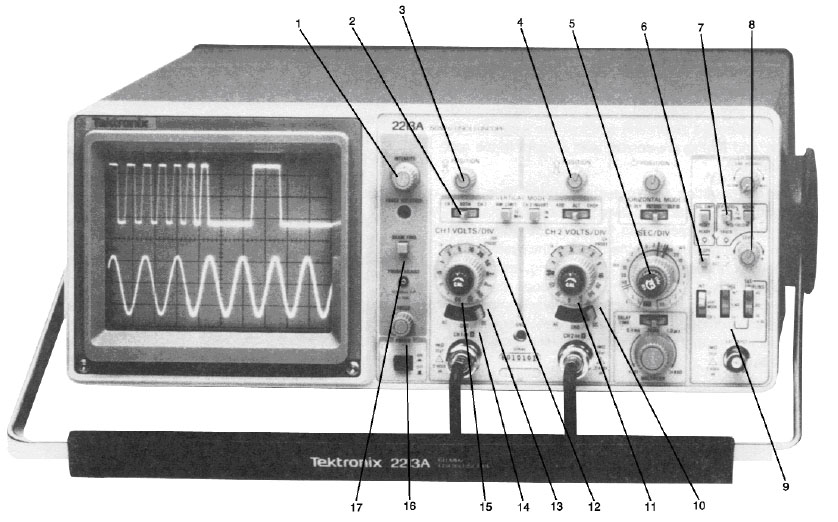
\includegraphics[width=.9\textwidth]{img/scope.jpg}\ec
		\end{minipage}
		\begin{minipage}{0.5\textwidth} 
			\captionsetup{width=0.8\textwidth}
			\caption[Image of a conventional oscilloscope.]{Image of a conventional oscilloscope.}\label{fig:scope}
		\end{minipage}\captionsetup{width=0.8\textwidth}
	\efi

		\subsubsection{Pulse Generator:}

This instrument simulates the pulses generated in the radiation detector and supplies the pulses with the known characteristics to the system entry. It is used for calibration, synchronization, etc. If used together, the oscilloscope and generator ensures that the electronics have been assembled according to the requirements of the experiment.

		\subsubsection{Discriminator:}

When a cosmic particle reaches the detector, the former will get mixed with the noise of the latter. Therefore, the signals output by both PMs must be filtered, by passing them through the \textbf{discriminator module}, where it will be required that the amplitude exceeds a certain threshold, in order to separate the produced particles that deposit more energy, such as the cosmic muons.

The module that performs this task is the discriminator, which accepts an analogue signal as input, whose amplitude and duration are dependent of the process that took place in the detector. The discriminator's output will be a logic signal with fixed height and duration (50 ns), and a rectangular shape, if the input signal has exceeded the discriminator's threshold. Each discriminator has two outputs: one is used to feed a counter that lets us know the number of pulses from each photomultiplier, and the other will address the coincidences module.

		\subsubsection{Coincidences module:}

The coincidences between the two detectors are evaluated using a NIM coincidence unit. This module has several inputs and one output. We will have an output signal when the input pulses overlap in time at least partially. Taking the output of this module to another counter we can accumulate the number of matches in a space of time.


		\subsubsection{Blocks and layers of absorbent material:}

There is a total of 20 layers of Al and 9 layers of Pb, with a thickness of 1.5 mm each.  The layers are not perfectly flat but can be bent. The Pb blocks are 5 cm thick.


		\subsection{Voltmeters}

The voltmeters used in the laboratory have a sensitivity of three and a half digits. They will be used to measure the voltage (HV) and the threshold voltage $V_{threshold}$. Therefore the error in measuring these quantities depends on the measurement scale used in each case [Appendix \ref{chap:app3}]. To measure, the value of the voltage is adjusted by turning a screw (potentiometer) and placing the terminal of the voltmeter to the corresponding measuring point. The proportionality constant of the voltmeter (which has a value of $\sqrt{2}$ since it measures effective values), ​​must also be considered.


		\subsection{Wiring}

Connections between linear and logic signals are made via standard BNC coaxial cables and connectors. The cables used to connect the two detectors with the coincidences module were of the same length so that the signal delay should be the same.


		\section{Determination of the working point}

To determine the operating point, the zone of maximum efficiency and stability of scintillators is searched. Once it is done for one, it is known for the other, since they are very similar. The high voltage (HV) and the threshold of the discriminator must be  properly adjusted.

	\graybox{1}{.9}{%
		\begin{description}
			\item[Problem] \hfill \\
				We want to detect the particles that have crossed both scintillators, any other signal is noise. This leads to the problem of determining the appropriate time window\footnote{In our case it corresponds to the time it takes a particle to travel the distance between the two scintillators.} of the detection system.
			\item[Solution:] \hfill \\
				To do this, we first have to know how fast the particles we want to detect travel. Muons, for example, are relativistic at ground level according to \cite{eid:04}. Since the distance between scintillators is $\sim$cm, this gives us a time window of  $\sim$ ns.
		\end{description}
		}

Since the total flux of cosmic rays at ground level is $J = 180 cm^{-2}s^{-1}$, the time window becomes: $\Delta T \ll 0.15 s$, as is calculated below. This gives an estimate of its value; but it is possible to determine it experimentally, defining:

	\be\label{eq:Qs} Q[s] = \frac{1}{2}\frac{N_{coinc}/t}{(N_1/t)(N_2/t)} \ee

It is found that when the number of counts is high, $Q = \Delta T$.


The value of the voltage is set to less than that recommended by the manufacturer for both scintillators, and the highest possible value for the discriminator is chosen. Measurements are taken sweeping the interval 1700--2300V in steps of 100V with one of the scintillators. $Q$ is calculated according to the above expression, and it is plotted against HV, where it is clear than it tends asymptotically to the value of the time window. This value is compared with the previous calculation.


	\subsection{Estimation of spurious coincidences}

	\graybox{1}{.9}{%
		\begin{description}
			\item[Issue:] \hfill \\
				Although the time window may be well adjusted, it is possible that randomly, two different particles arrive each at a different detector inside the time  window (or that the noise in both detectors generates a coincidence) and then the system will assume it as a real coincidence.
			\item[Solution:] \hfill \\
				The frequency of random coincidence events is proportional to the coincidences window size and to the number of individual counts on each detector, \textit{i.e.}:

\noindent\be Random\ coincidences: \frac{N_{rand}}{t} = \frac{N_1}{t}\frac{N_2}{t}2\Delta T\label{eq:random}\ee
		\end{description}
	}

Once the time window is determined, the spurious contribution can be obtained making this simple calculation.

With the flux $J$ obtained at ground level, if $S$ is the surface of the detector, the average rate of particles in each detector is given by $N / t = J · S$ = 180 $m^{-2}s^{-1}\times$0.031$m^{-2}$ = 6 particles per second. If it is imperative that $N_{rand} / t \ll N / t$, and the above expression is used, we obtain $\Delta T \ll 0.15 s$, as discussed above.


	\subsection{Determination of the plateau by changing the high voltage}

	\fcolorbox{lightgray}{lightgray!50!white}{
		\parbox{\textwidth}{

			\bc\parbox{.9\textwidth}{
	\begin{description}
		\item[Issue:] \hfill \\ The detector does not behave the same way for all voltages. If the HV voltage is very small, the signal strength is small and falls below the threshold, so it is not registered. If the HV is high, we have a considerable contribution of detector noise (see \enquote{\textit{	Set up and instrumentation: Scintillators and photomultipliers}}). What we want is an intermediate situation.
		\item[Solution:] \hfill \\ Several measurements are realized between 1700 and 2300 HV V as in the previous section. Initially the thresholds are set to their minimum values ​​(-35 mV), so that all the signals from the detectors are received. Then the signals from each detector and the coincidences are noted. As the noise is expected to be high, it is expected that the number of counts of each detector (ray + noise) will be greater than the number of coincidences (rays).
	\end{description}
			}\ec
		}%
	} \par



If the coincidences are plotted against the HV, a substantially constant, flat area called \textit{plateau} will appear, which allow us to determine the operating point of the detectors. If random coincidences are also included in the same graph, there will be another curve that will give us information on the voltage at which these coincidences start contributing.


	\subsection{Determination of the plateau by changing the threshold}

The operating voltage is set to the manufacturer's recommended value,  and the threshold is set to the maximum ($-$400 mV). Then it is reduced  in steps of 50 mV until the minimum is reached ($-$35 mV). By raising the detector's threshold, a reduction in the difference between the number of coincidences and individual signals must be observed, because noise is mainly discriminated.

	\section{Statistical characterization of cosmic radiation}

According to the theory of probability, if a distribution function is known, every moment of it is known too. Conversely, if a distribution of all moments are known, this is equivalent to knowing the distribution. Therefore to determine a probability distribution associated with an experiment, there are two alternatives: either to determine the distribution or to determine all its moments (or at least the most relevant).

When the number of occurrences of a measure is very small, the probability distribution fits well to a Poisson distribution (Appendix \ref{sec:poisson}). Radioactive decay (in the present case, the primary particles decaying into the secondary, which are the ones of interest here) is a random process that obeys the Poisson distribution, according to which the standard deviation of the distribution with media $\mu$ is $\sqrt{\mu}$ (Appendix \ref{sec:poisson}).

However, when the number of counts is greater, data starts to progressively conform to a Gaussian distribution. Therefore, the procedure is to make measurements in intervals of 5s for one hour, to have something of the order of about 3 counts, and then repeat the same measurement every 10s and 20s. With the values ​​obtained, a histogram of the number of coincidences counted in each measure is plotted. Then it is found that the data represented in the histogram follows a Poisson distribution in the first case, while in the second and third case it follows a Gaussian distribution. The goodness of fit is evaluated with a $\chi^2$ test.


	\subsection{Modelling of the quality of experimental data and settings: Chi square test}

Through the minimization process known as the \textit{least squares method}, we can determine the value of a theoretical parameter function $f(x, a_1, ..., a_m)$ which is fitted to a set of $n$ experimental points $f (x_i; y_i)$.

The method states that the best values ​​of the $a_j$ are those for which the function


	\be\chi^2 = \sum_i^n\frac{\left(y_i-f(x_i;a_j)\right)^2}{\sigma_i^2}\ee

is minimal, which is usually calculated by numerical methods.

Suppose a set of $n$ random events that follow Poisson and Gauss and appear with frequencies $e_i$. Let $N = \sum e_i$ be the number of expected frequencies. Then the probability of observing the event $i$ is $e_i/N$, and it represents the fraction of cases in which we would see it if we repeated the experiment infinite times. Thus we obtain:

			\noindent\be\chi^2 = \sum_i^n\frac{\left(o_i-e_i\right)^2}{e_i}\ee

where $e_i$ are the theoretical frequencies and $o_i$ are the experimental ones.

Limitation: If all $o_i$ are greater than $e_i$ is not possible to say that the agreement is very good even if $\chi^2$ is small. This method is not a universal panacea.

The procedure is as follows: the number of events occurring in each area of probability is compared with the number of expected events. If the difference is small (of the order of the expected fluctuations, i.e., $\sim \sqrt{e_i} = \sigma_i$), there is a good agreement between experimental and theoretical data (Appendix \ref{sec:chi2}), i.e., if $\chi^2 < \nu$ there is agreement, and if $\chi^2 \gg \nu$, there is not, where $\nu$ represents the degrees of freedom of the system.



\subsection{Separation of the hard component of coincidences}\label{sub:separation}


Recalling the equations \ref{eq:in}, \ref{eq:in2} and \ref{eq:ipi} in the  theoretical introduction chapter, we see that each particle is attenuated differently in the atmosphere depending on their energy.

With our experimental set-up we can not measure the number of coincidences as a function of energy, but we measure the number of coincidences averaged over all energies. However, with the help of the oscilloscope and without altering anything, we could determine the energy distribution of the incident particles, simply by connecting the detector to the oscilloscope and measuring the amplitude of the signals appearing (for this you may want to freeze the image in the oscilloscope with many reflections).

Some definitions are important here:

\bi
	\item \textit{Linear absorption coefficient} ($\mu$): variable indicating the ability of a material as an absorber. In g cm$^{-2}$.
	\item \textit{Mass absorption coefficient ($\Lambda$)}: The linear absorption coefficient divided by the density ($\rho$) of the absorbent in g cm$^{-3}$ is often expressed as $\mu / \rho$ and units are usually given in cm.
	\item \textit{Stopping power ($dE / dx$)}: Measurement of the effect of a substance on the kinetic energy of a charged particle passing through. It is typically given in MeV / cm.
\ei


It also important to introduce the typical exponential decay law: given a certain flux of particles with a certain kinetic energy, the number of them passing through a material of increasing thickness typically follows an exponential decay function given by:

		
		\be-\frac{dN(x)}{dx} = \mu N(x) \quad \rightarrow \quad \int_{N_0}^{N(x)}\frac{dN(x')}{N(x')} = - \mu\int_0^x dx' \ee
		\bc $N(x) = N(0) e^{-\mu x}$ \ec
		\be N(x) = N(0) e^{\frac{-x\rho}{\Lambda}}\ee

where $N(x)$ is the number of particles of the incident beam that \enquote{survive} at a depth $x$ of the material, $\mu$ is the \enquote{coefficient of linear absorption} of such particles in the material, and $N (0)$ is the number of particles that hit the material initially.

Since $\Lambda$ is a characteristic parameter of the radiation, the attenuation coefficient depends on the particle type; given a particular material, the absorption coefficient $\mu$ is smaller in the case of muons than in the case of the soft component, because $\Lambda$ is greater.

As in air it would be difficult to stop them with the measurement system used\footnote{In air the values ​​are: $\Lambda_{soft}$ = 100 g cm$^{-2}$ and $\Lambda_{hard}$ = 1500 g cm$^{-2}$, which give typical values ​​of 150 Km for muons in air, and 10 km for electrons.}, higher intensities are mitigated with elements such as Pb and Al:

\bc$\rho_\text{Pb}$ = 11.340 g cm$^{-3}$\\[12pt]
  $\rho_\text{Al}$  = 2.700 g cm$^{-3}$\ec

The procedure is as follows: the Al plates are placed between the two scintillators and then the number of layers is increased to the maximum, up to a thickness of about 30 cm. The same is done for Pb, but in combination with the blocks, in order to get more intermediate thicknesses.

Once these measurements are made, we proceed to calculate $\Lambda$ for Pb and Al by plotting the coincidences against the thickness. The plot can be fitted to the exponential attenuation equation, or we can take logarithms and fit to a straight line.

In the case of Al the slope is smoother for the soft component that in the case of Pb, where there are two distinct slopes. The first of them is abrupt and the second is less steep. This is because when reaching a certain thickness of Pb, the soft component is no longer able to cross it, and only the hard one penetrates. This, and the fact that both components have a well defined energy, justify that in the case of Pb a fit to the sum of two exponentials is done. Furthermore, from the fit, the values of the hard and soft components can be extrapolated to zero thickness.

Once the hard and soft components are separated, we would know the number of $\mu^\pm$ and $e^\pm$ at zero thickness, so it would be possible to compare this experimental value with the theoretical predicted value. The theoretically predicted value for the total flux of cosmic radiation per unit area and per unit time is: $J$ = 180 cm$^{-2}$ s$^{-1}$ = 130 cm$^{-2}$ s$^{-1}$ (hard) + 50 cm$^{-2}$ s$^{-1}$ (soft).



\section{Calculation of the geometric efficiency}


This section will attempt to evaluate the geometric efficiency of the measurement system used, which is related to the fact that the detectors, due to the fact that  they are at a certain distance from each other, do not provide the same number of coincidences for different separation distances, but instead there are losses due to the geometry of the assembly.

To estimate its value, both scintillators are placed at zero distance from each other and coincidences are recorded. From the previous section where scintillators were at a distance, we can determine the fraction of muons contributing to the total counts, and multiply the result by the total active area, to verify that a compatible value is not obtained, due to the effect of efficiency.

Then we will separate the detectors and will take note of the number of coincidences obtained at each distance. Appendix \ref{chap:app1} shows how to calculate the flux integral which allows to obtain $I$, the intensity of particles per unit time in a rectangular detector geometry, which in the present case will be the flux measured on the upper detector.

Since in this section coincidences are measured, the measured $I$ is dependent on the efficacy with which it completely arrives at the second detector, which in turn depends on the distance between scintillators. If scintillators are separated a distance $d$, a diminishing flux is measured that follows the relationship:

\be I(d) = \epsilon (d) I = \frac{N_{coinc}(d)}{t}\ee

where $\epsilon (d)$ is the geometric efficiency.

You may evaluate this $\epsilon (d)$ in two different ways and then compare them:

\bi
	\item Calculating (from experimental coincidence data) the ratio:
\be\frac{N_{coinc}(d)}{N_{coinc}}\ee
	\item Performing a Monte Carlo simulation, as described in  Appendix \ref{chap:app2}.
\ei

Finally, assuming that the soft radiation has the same angular distribution as the hard one, we can represent the relative fraction of hard and soft component as a function of the distance between scintillators, and if all goes well, it should be approximately constant.





\subsection{Comparison of experimental results of the flux with the tabulated values}


The goal of this section is to determine the contribution of the hard component at a given distance with the help of section \ref{sub:separation} about the separation of the hard component, to calculate the geometric correction (MC) for that distance and finally multiply by the area.

After calculating the efficiency, we can calculate $J_0$ (Appendix \ref{chap:app1}) from the value of the number of coincidences due to the hard component, calculated in the previous section. The uncertainty in the value of $J_0$ should also be calculated, and its sources specified.

The theoretical values ​​used as reference are listed below:

	\ctable [
	cap	    = {Typical values ​​obtained with the Monte Carlo simulation.},
 	caption = {Typical values obtained with the Monte Carlo simulation as a function of the smaller (a) and larger (b) sides of the detectors, and the separation (d) between the two.},
 	label = {tab:montecarlo},
 	pos	  = H,
	botcap
	]
	{c c c c}
	{}
 	{\FL
		\textbf{a (cm)} & 
		\textbf{b (cm)} & 
		\textbf{d (cm)} & 
		\textbf{\pbox{7cm}{\pcen Fraction that crosses both detectors (\%)}}  \\
		27 & 9 & 26 & 15 \\
		28 & 10 & 24 & 19 \\
		29 & 11 & 22 & 23 
	\LL}





	\ctable [
	cap	 = {Tabulated values ​​of RPPP.},
 	caption = {Tabulated values taken from \cite{prd:96}},
 	label   = {tab:rppp},
 	pos	 = H,
	botcap
	]
	{c c c c}
	{}
 	{\FL
		&
		\textbf{Total} &
		\textbf{Hard component ($\sim \mu^+$)} &
		\textbf{Soft component ($\sim e^+$)}\\
		$J_0 (m^{-2}s^{-1}sr^{-1})$ & 110 	& 80 							& 30 \\
		$J (m^{-2}s^{-1})$ 			& 180 	& 130 							& 50
	\LL}\vfill





	\graybox{.8}{.65}{
		\bc\textcolor{gray}{\Large{\sffamily General comments for all sections:}}\ec

\noindent\bi
	\item You should always work with the number of counts per unit time.
	\item While measuring, scintillators should always be covered with a black cloth or similar, to avoid light contributions from the laboratory or otherwise.
	\item When the number of counts is very high, the \enquote{x100} option in the coincidence module can be used.
	\item Always keep the scintillators as aligned as possible.
	\item It's recommended to wait a reasonable time during the acquisition, so that the number of counts measured has a statistical error that is consistent and its value is kept under 5\%.
\ei\vspace{2ex}
	}

The next chapter will hopefully help you know the order of the values you must get when measuring.
